\documentclass[pageno]{jpaper}
%\newcommand{\iscasubmissionnumber}{117}

\usepackage[normalem]{ulem}
\usepackage{booktabs}
\usepackage{mathtools}
\usepackage{ragged2e}
\usepackage{rotating}
\usepackage{array}
\usepackage{grffile}

\usepackage{epsfig}
\usepackage{float}
\usepackage{wrapfig}
\usepackage{setspace}
\usepackage{multirow}
\usepackage{graphicx}
\usepackage{fancyhdr}
%\usepackage{paralist}
%\usepackage{capt-of}

\usepackage{color}
\usepackage{xcolor,colortbl}
\usepackage{chngpage}
\usepackage{enumitem}
\usepackage{enumerate}
\usepackage{amsmath,relsize}
\usepackage[justification=centering]{caption}
\usepackage{tabu}
\usepackage{stmaryrd} % short right arrow

\usepackage{listings}
\usepackage[makeroom]{cancel}


\usepackage{amssymb}% http://ctan.org/pkg/amssymb
\usepackage{pifont}% http://ctan.org/pkg/pifont
\usepackage[nomargin,inline,draft]{fixme}
\newcommand{\cm} {\clap{\small\ding{51}}\small\hphantom{--}}
\newcommand{\cmi}{\clap{\small\ding{51}-}\small\hphantom{--}}%
%\newcommand{\xm} {\clap{\ding{55}}\hphantom{--}}
\newcommand{\xm} {\clap{\small}\small\hphantom{--}}

\newcommand{\Forall}{\displaystyle\mathop\mathlarger{\mathlarger{\mathlarger{\forall}}} } 

%\newcommand{\cm} {{Y}}%
%\newcommand{\cmi}{{P}}%
%\newcommand{\xm} {{}}%


\usepackage{tikz,array}
\usetikzlibrary{calc}

%\newcommand*\circled[1]{\tikz[baseline=(char.base)]{
%            \node[shape=circle,draw,inner sep=2pt] (char) {#1};}}

%\newcommand*\ccircled[1]{\tikz[baseline=(char.base)]{
%            \node[shape=circle,draw,inner sep=2pt] (char) {#1};}}

\tikzstyle{every node}=[font=\footnotesize]

\newcommand{\hcancel}[5]{%
    \tikz[baseline=(tocancel.base)]{
        \node[inner sep=0pt,outer sep=0pt] (tocancel) {#1};
        \draw[black] ($(tocancel.south west)+(#2,#3)$) -- ($(tocancel.north east)+(#4,#5)$);
    }%
}%

\newcommand*\circled[1]{\tikz[baseline=(char.base)]{
            \node[shape=circle,draw,inner sep=0.5pt, minimum size=0.24cm] (char) {#1\vphantom{H}};}}

\newcommand*\ccircled[1]{\hcancel{\tikz[baseline=(char.base)]{
            \node[shape=circle,draw,inner sep=0.4pt, minimum size=0.24cm] (char) {#1\vphantom{H}};}}{-1pt}{1pt}{1pt}{-1pt} }


\begin{document}
\title{
\vspace{-0.15in}
An Efficient GPGPU Implementation of Viola-Jones Classifier Based Face Detection Algorithm
\vspace{-0.15in}
}





\author{Sharmila Shridhar  \\ \and  
    Ramsai Manoj Bamdhamravuri  \\ \and 
        Vinay Gangadhar 	\\ \and
            \{sshridhar, bamdhamravur, gangadhar\}@wisc.edu} 

\date{}
\maketitle

%\thispagestyle{empty}
\begin{abstract}
   
\vspace{0.1in}

Applications with large amount of data level parallelism
can benefit from General Purpose based Graphics Processing
Units (GPGPUs) because of better energy efficiency and performance compared to a CPU. Due to GPGPUs’ impressive
computing throughput and memory bandwidth, many applications with enough parallelism can take advantage of acceleration using GPGPU. Computer vision algorithms are one such
workload domain which can better utilize the large number
of cores in GPU, and hence meet their real-time requirements
of the applications. One such application is \emph{Face Detection}
which has real-time constraint on its execution. Sequential
processing of image windows with image downsampling and classifiers on CPU is difficult to meet the real-time requirements. 

In this project, we have
implemented the face detection acceleration algorithm based
on Viola-Jones cascade classifier on the GPGPU CUDA platform.
We have considered different portions of the viola jones algorithm which include 
\emph{nearest neighbor}, \emph{integral image} and {HAAR classifier} that can
be parallelized.
We identify different bottlenecks in GPU implementation and include optimizations
which gives the performance benefit. We explain each of these optimizations in detail for all the kernels. 
We finally compare the execution of the same algorithm executed
on the CPU and analyze the gains from the GPU.
We achieve a speedup upto 5.35x (including the inclusive time) compared to the single threaded performance of CPU.




\end{abstract}

\section{Motivation}\label{sec:motivation}


In this project, we intend to implement face detection algorithm based on the Viola Jones classifier \fixme{ref} on GPU. 
As a starting point, we take the GNU licensed C++ program that has the 
algorithm implemented to detect faces in images \fixme{ref}. 
There are various portions in the algorithm that can be parallelized and hence can leverage the hardware of GPU efficiently. 
Section 1 explains Viola Jones algorithm briefly. Section 2 explains the portions we are going to parallelize and offload to the GPU.


Viola Jones Face Detection Algorithm
The algorithm has four stages:
Haar feature selection: The Viola Jones classifier method is based on Haar-like features. 
The features consist of white and black rectangles as shown in Fig 1. 
These features can be thought of as pixel intensity evaluation sets. 
For each feature, we subtract black region’s pixel value sum from white region’s pixel value sum. 
If this sum is greater than some threshold, it is decided that the region has this feature. 
This is the characteristic value of a feature. We have the Haar features
to be used for face detection

 
\section{Face Detection Background}\label{sec:arch}


Figure~\ref{fig:haar} gives a high level overview of the PENN architecture 

\begin{figure}[h]
  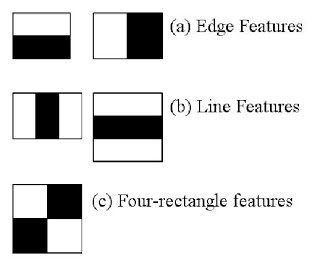
\includegraphics[width=0.45\linewidth]{figs/haar.jpg}
  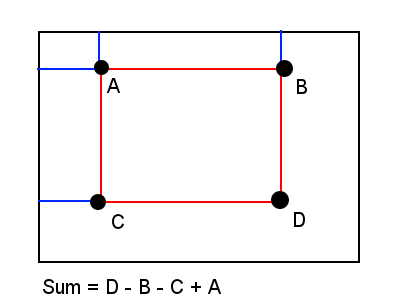
\includegraphics[width=0.45\linewidth]{figs/sum.png}
  \caption{Four kinds of HAAR feature rectangles \textnormal{\small }  }
  \label{fig:penn-fabric}
\end{figure}


Figure~\ref{fig:add-table} gives a high level overview of the PENN architecture 

\begin{figure*}
  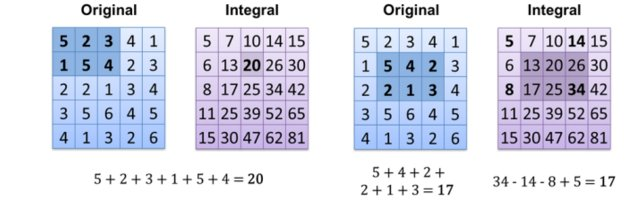
\includegraphics[width=0.9\linewidth]{figs/add.jpg}
  \caption{Four kinds of HAAR feature rectangles \textnormal{\small }  }
  \label{fig:add-table}
\end{figure*}


\section{Evaluation framework}\label{sec:evaluation}
For this project, we evaluate the performance of GPU implementation with that of CPU.
There is no training involved. Haar features, number of features in each stage are already determined.
We compare the execution time for face detection in an image on CPU and on GPU. As mentioned in Methodology section, we
parallilize three different portions in the algorithm. We will analyze the contribution of each of
the three sections parallelized for performance implications.
Since sufficient parallelism can be extracted in this image processing application, we hope to get
better performance on GPU.


\section{Project phases}\label{sec:plan}

We explain the phases of project here and expected timeline for 
each step. Some of the phases can be carried out in parallel and will be distributed 
among the project members.

\begin{itemize}
\item \textbf{Phase 0 [1 week]:} Choose the representative workloads/ kernels of neural network domain
targeting different applications (image processing, speech recognition, text parsing etc.,). 
Use the trace based modeling tool TDG (~\cite{tonytdg}) modeled
for PENN to determine the initial performance and power estimates for each kernel.
More accurate analysis of workloads (profiling) to be done here and see if there are any missing architectural
pieces not considered for current PENN architecture.

\item \textbf{Phase 1 [2 days]:} Based on phase 0 analysis, some important design trade-off decisions should be taken. Those steps are listed here:
i) Low-power core: Properties (pipeline stages, memory interface and hierarchy etc.,) of low-power core which does the co-ordination.
Compiler and software toolchain for the core (RISCV toolchain and their in-order core can be a good start). 
ii) CGRA: Types of problem specific FUs inside the fabric.  Interface to low-power core and scratchpad memory.
Addressing of scratchpad space and global memory. Scheduling pattern for CGRA. Scratchpad size and bit-width.
iii) Programming model: API for PENN. Pragmas and code annotations for compilation.

\item \textbf{Phase 2 [3 weeks]:} This phase involves implementation of individual modules of PENN listed in Phase 1. 
Implementation of low power core and CGRA in Verilog and C++.
Writing API routines for PENN and compiler support (Note: A full-fledged compiler may not be implemented but 
a framework to generate instructions and configuration stream will be implemented.)
Tools needed for the project are explained in Section~\ref{sec:meth}.

\item \textbf{Phase 3 [1 week]:}This phase mainly involves evaluating implemented synthesized PENN architecture with
    representative workloads chosen in Phase 0. We also use C++ simulator written for PENN to correlate the functionality of the synthesized version. 
We plan to evaluate PENN for performance, area and power against a state-of-the-art DSA for Neural Network.

\item \textbf{Phase 4 [2 weeks]:} This phase mainly involves prototyping PENN on Zynq FPGA. However, this phase will be realized only if Phase 3 is
    completed well within course project time limit. Project report is also part of this phase.
\end{itemize}




 
\section{Methodology }\label{sec:meth}
<<<<<<< HEAD

=======
We try to list out some of the tools we are considering for our project and also the methodologies involved with those.

We plan to use existing RISCV LLVM toochain~\cite{nguyenlinux} as part of compiler framework. 
For low power core, we are considering a three stage pipeline SODOR core as it is power efficient compared to any standard VLIW core. 
For implementing individual modules, we want to use CHISEL~\cite{chisel2012} tool, which uses an embedded scala language to generate verilog code and C++ simulator
framework. Also, for our initial modeling phase, we used a trace based modeling tool TDG and we will be using the same for our further analysis.   

For evaluating PENN, we will be collecting performance, power and area statistics of the synthesized version and compare it with statistics 
given in the literature of DSA papers. 
>>>>>>> 49ddcfc99c241d091550ef080d974a6076980d94

\section{Related Work}\label{sec:related}


%\input{architecture}
%\input{compiler}
%\input{methodology}

\bstctlcite{bstctl:etal, bstctl:nodash, bstctl:simpurl}
\bibliographystyle{IEEEtranS}
\bibliography{main}

\end{document}
